\documentclass[12pt]{article}
\usepackage[paperwidth=25cm,paperheight=17cm,margin=1.4cm]{geometry}
\usepackage[T1]{fontenc}
\usepackage[utf8]{inputenc}
\usepackage[magyar]{babel}
\usepackage{lmodern}
\usepackage{amsmath}
\usepackage{enumitem}
\usepackage{array}
\usepackage{tikz}
\usetikzlibrary{arrows.meta,decorations.pathmorphing}
\usepackage{pgfplots}
\pgfplotsset{compat=1.16}
\usepackage[most]{tcolorbox}

\pagestyle{empty}
\setlength{\parindent}{0pt}
\setlength{\parskip}{4pt}
\setlist[itemize]{leftmargin=1.4em, itemsep=3pt, topsep=2pt, parsep=0pt}

\newcommand{\dia}[1]{\newpage{\Large\bfseries #1}\par\vspace{2pt}{\color{blue!50!black}\hrule height 1pt}\vspace{8pt}}

\newtcolorbox{pelda}[1][]{colback=green!4,colframe=green!45!black,fonttitle=\bfseries,
  title=Kidolgozott példa,left=5pt,right=5pt,top=3pt,bottom=3pt,before skip=6pt,after skip=4pt,#1}
\newtcolorbox{fontos}[1][]{colback=blue!3,colframe=blue!45!black,
  left=5pt,right=5pt,top=3pt,bottom=3pt,before skip=6pt,after skip=4pt,#1}

% látható színkép: 380 nm -> 25bp, 750 nm -> 75bp
\pgfdeclarehorizontalshading{lathato}{100bp}{
  color(0bp)=(violet!80!black); color(25bp)=(violet!80!black); color(33bp)=(blue);
  color(40bp)=(cyan); color(45bp)=(green!80!black); color(52bp)=(yellow);
  color(56bp)=(orange); color(62bp)=(red); color(75bp)=(red!60!black); color(100bp)=(red!60!black)}

% véletlen pontfelhő: #1 próbálkozás, #2 mag, #3 valószínűség (\x,\y-ból)
\newcommand{\felho}[3]{%
  \pgfmathsetseed{#2}
  \foreach \i in {1,...,#1}{
    \pgfmathsetmacro{\x}{1.3*rand}
    \pgfmathsetmacro{\y}{1.3*rand}
    \pgfmathsetmacro{\p}{#3}
    \pgfmathsetmacro{\u}{rnd}
    \ifdim \u pt < \p pt \fill[blue!70!black] (\x,\y) circle (0.5pt); \fi
  }}

\begin{document}

%====================================================================
\begin{center}
  \vspace*{0.8cm}
  {\Huge\bfseries Az atom szerkezete}\\[8pt]
  {\Large Az atommodellek története a kísérletek tükrében}\\[1.2cm]
\end{center}

\begin{center}
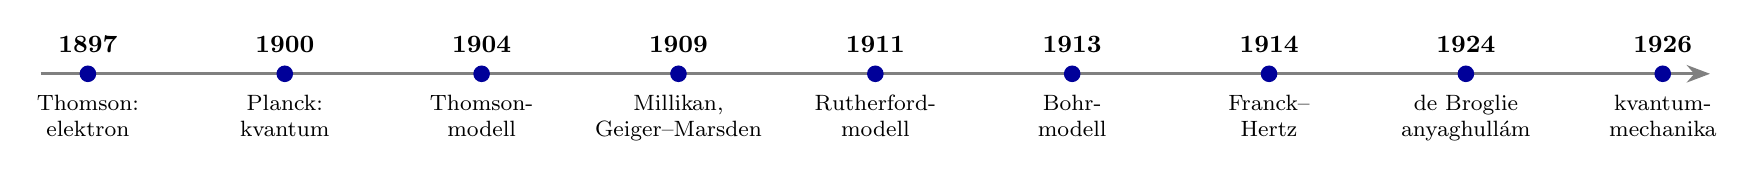
\begin{tikzpicture}[font=\small,>=Stealth]
  \draw[->,very thick,gray] (-0.6,0) -- (20.6,0);
  \foreach \x/\ev/\fent/\lent in {
      0/1897/{Thomson:}/{elektron},
      2.5/1900/{Planck:}/{kvantum},
      5.0/1904/{Thomson-}/{modell},
      7.5/1909/{Millikan,}/{Geiger--Marsden},
      10.0/1911/{Rutherford-}/{modell},
      12.5/1913/{Bohr-}/{modell},
      15.0/1914/{Franck--}/{Hertz},
      17.5/1924/{de Broglie}/{anyaghullám},
      20.0/1926/{kvantum-}/{mechanika}}{
    \fill[blue!60!black] (\x,0) circle (3pt);
    \node[above=4pt,font=\bfseries\small] at (\x,0) {\ev};
    \node[below=4pt,align=center,font=\footnotesize] at (\x,0) {\fent\\\lent};
  }
\end{tikzpicture}
\end{center}

\vspace{0.8cm}
\begin{center}
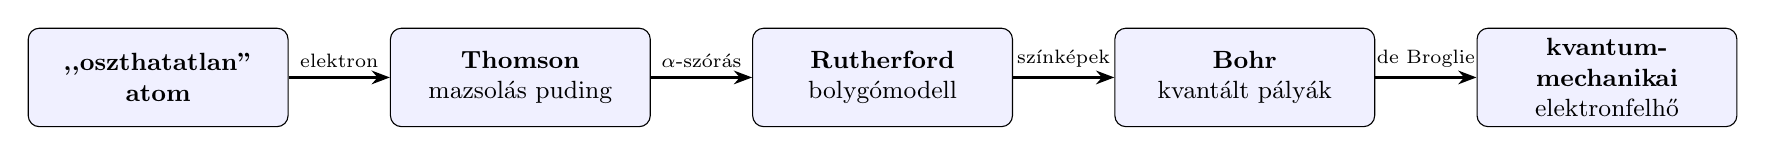
\begin{tikzpicture}[font=\small,
    modell/.style={draw,rounded corners,fill=blue!6,minimum width=3.3cm,minimum height=1.25cm,align=center},
    >=Stealth]
  \node[modell] (a) at (0,0)    {\textbf{,,oszthatatlan''}\\\textbf{atom}};
  \node[modell] (b) at (4.6,0)  {\textbf{Thomson}\\mazsolás puding};
  \node[modell] (c) at (9.2,0)  {\textbf{Rutherford}\\bolygómodell};
  \node[modell] (d) at (13.8,0) {\textbf{Bohr}\\kvantált pályák};
  \node[modell] (e) at (18.4,0) {\textbf{kvantum-}\\\textbf{mechanikai}\\elektronfelhő};
  \draw[->,thick] (a) -- node[above,font=\scriptsize] {elektron} (b);
  \draw[->,thick] (b) -- node[above,font=\scriptsize] {$\alpha$-szórás} (c);
  \draw[->,thick] (c) -- node[above,font=\scriptsize] {színképek} (d);
  \draw[->,thick] (d) -- node[above,font=\scriptsize] {de Broglie} (e);
\end{tikzpicture}
\end{center}

\vspace{0.8cm}
\begin{center}
\fbox{\parbox{0.92\textwidth}{\centering
  $h = 6{,}63\cdot 10^{-34}~\text{J}\cdot\text{s}$, \;
  $e = 1{,}6\cdot 10^{-19}~\text{C}$, \;
  $m_e = 9{,}1\cdot 10^{-31}~\text{kg}$, \;
  $k = 9\cdot 10^{9}~\tfrac{\text{N}\cdot\text{m}^2}{\text{C}^2}$, \;
  $1~\text{eV} = 1{,}6\cdot 10^{-19}~\text{J}$, \;
  $hc \approx 1240~\text{eV}\cdot\text{nm}$}}
\end{center}

%====================================================================
\dia{1. 1900: ,,két felhő'' a fizika egén}

\begin{minipage}[t]{0.52\linewidth}\vspace{0pt}
\begin{itemize}
  \item 1900 körül a fizikusok úgy érezték, a fizika szinte kész: a mechanika, a hőtan és
    az elektromágnesség mindent megmagyaráz. Lord Kelvin egy előadásában csak két
    ,,felhőt'' említett a fizika egén. Az egyikből a relativitáselmélet, a másikból a
    \textbf{kvantumfizika} nőtt ki.
  \item \textbf{Ultraibolya katasztrófa:} a klasszikus fizika (Rayleigh--Jeans-törvény) szerint
    egy izzó test sugárzása a rövid hullámhosszak felé \emph{a végtelenbe nő}. Eszerint
    minden meleg test végtelen energiát sugározna ki az ultraibolyában -- ez nyilvánvalóan
    képtelenség.
  \item \textbf{Planck (1900)} megoldása (előző óra): az energia csak $E = hf$ adagokban
    sugározható ki. A nagy frekvenciás (UV) adagok ,,drágák'', ezért ott a sugárzás
    elhal.
\end{itemize}
\begin{fontos}
\textbf{A kérdés, amivel ma foglalkozunk:} ha az energia adagos, \emph{mi az atomban} az,
ami ezeket az adagokat kibocsátja? Ehhez tudni kell, hogyan épül fel az atom.
\end{fontos}
\end{minipage}\hfill
\begin{minipage}[t]{0.45\linewidth}\vspace{0pt}\centering
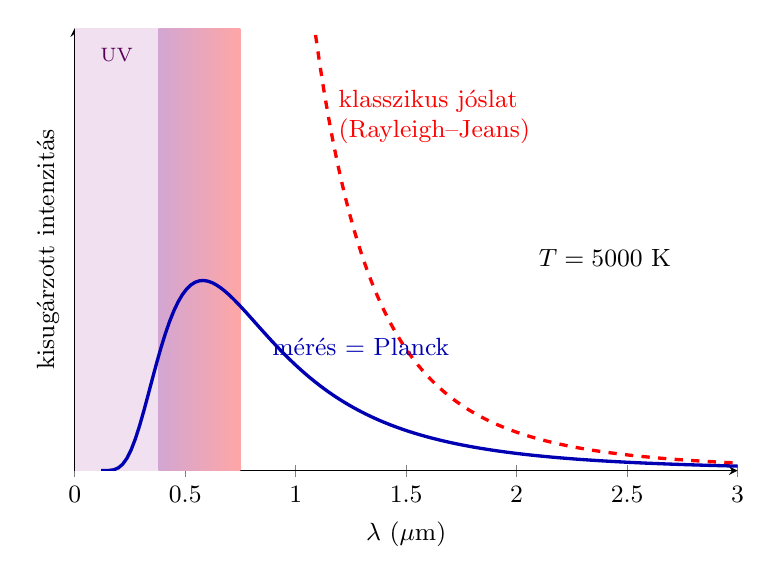
\begin{tikzpicture}
\begin{axis}[width=10cm,height=7.2cm,xmin=0,xmax=3,ymin=0,ymax=0.25,
    xlabel={$\lambda$ ($\mu$m)},ylabel={kisugárzott intenzitás},
    yticklabels={},ytick=\empty,
    tick label style={font=\small},label style={font=\small},
    axis lines=left,clip=true]
  \fill[violet!12] (axis cs:0,0) rectangle (axis cs:0.38,0.25);
  \node[font=\scriptsize,violet!70!black] at (axis cs:0.19,0.235) {UV};
  \fill[left color=violet!35,right color=red!35] (axis cs:0.38,0) rectangle (axis cs:0.75,0.25);
  \addplot[very thick,blue!70!black,domain=0.12:3,samples=150]
    {1/(x^5*(exp(14388/(x*5000))-1))};
  \addplot[very thick,red,dashed,domain=1.09:3,samples=100]
    {5000/(14388*x^4)};
  \node[font=\small,red,anchor=west,align=left] at (axis cs:1.15,0.2) {klasszikus jóslat\\(Rayleigh--Jeans)};
  \node[font=\small,blue!70!black,anchor=west,align=left] at (axis cs:0.85,0.07) {mérés = Planck};
  \node[font=\small] at (axis cs:2.4,0.12) {$T = 5000$~K};
\end{axis}
\end{tikzpicture}
\end{minipage}

%====================================================================
\dia{2. Katódsugárzás: az elektron felfedezése (Thomson, 1897)}

\begin{minipage}[t]{0.55\linewidth}\vspace{0pt}
\begin{itemize}
  \item Ritkított gázzal töltött csőben a negatív elektródából (\textbf{katódból})
    láthatatlan sugárzás indul ki: a \textbf{katódsugárzás}. Az üveg ott világít, ahol
    eltalálja.
  \item \textbf{J.\,J.\ Thomson} megmutatta, hogy a sugarak elektromos és mágneses térben
    is \textbf{eltérülnek}, mégpedig úgy, ahogy \textbf{negatív töltésű részecskék}.
  \item Megmérte a részecskék \textbf{fajlagos töltését} ($e/m$, töltés per tömeg):
    \[ \frac{e}{m} \approx 1{,}76\cdot 10^{11}~\frac{\text{C}}{\text{kg}} \]
    Ez kb.\ \textbf{1800-szor} nagyobb, mint a legkönnyebb ionra, a hidrogénionra, és
    \emph{minden katódanyagra ugyanannyi}.
\end{itemize}
\begin{fontos}
\textbf{Következtetés:} létezik egy, az atomnál jóval könnyebb, negatív részecske, az
\textbf{elektron}, és ez minden atomban megtalálható. Az atom tehát \emph{nem
oszthatatlan}: van belső szerkezete.
\end{fontos}
\end{minipage}\hfill
\begin{minipage}[t]{0.42\linewidth}\vspace{0pt}\centering
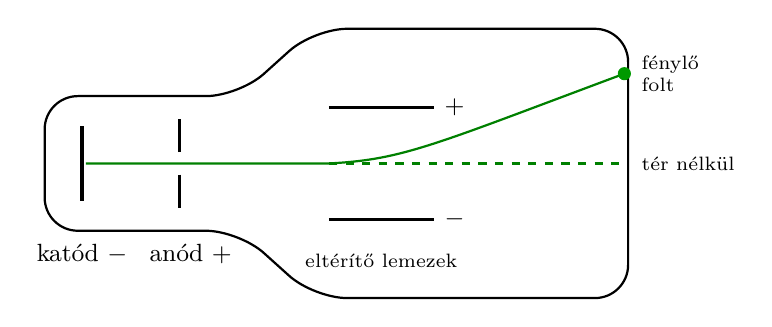
\begin{tikzpicture}[scale=0.95,>=Stealth,font=\small]
  \draw[thick,rounded corners=12pt] (-0.4,-0.9) -- (2.2,-0.9) -- (3.2,-1.8) -- (7.4,-1.8)
    -- (7.4,1.8) -- (3.2,1.8) -- (2.2,0.9) -- (-0.4,0.9) -- cycle;
  \draw[very thick] (0.1,-0.5) -- (0.1,0.5);
  \node[below] at (0.1,-0.95) {katód $-$};
  \draw[very thick] (1.4,0.15) -- (1.4,0.6);
  \draw[very thick] (1.4,-0.15) -- (1.4,-0.6);
  \node[below] at (1.55,-0.95) {anód $+$};
  \draw[very thick] (3.4,0.75) -- (4.8,0.75) node[right] {$+$};
  \draw[very thick] (3.4,-0.75) -- (4.8,-0.75) node[right] {$-$};
  \draw[thick,green!50!black] (0.15,0) -- (3.4,0) .. controls (4.4,0.05) and (4.8,0.25) .. (7.35,1.2);
  \draw[thick,green!50!black,dashed] (3.4,0) -- (7.35,0);
  \fill[green!60!black] (7.35,1.2) circle (2.5pt);
  \node[right,align=left,font=\scriptsize] at (7.45,1.2) {fénylő\\folt};
  \node[right,font=\scriptsize] at (7.45,0) {tér nélkül};
  \node[font=\scriptsize] at (4.1,-1.3) {eltérítő lemezek};
\end{tikzpicture}

\vspace{6pt}
\begin{pelda}[title=Iskolai mérés: fonalsugárcső]
Az $U$ feszültséggel gyorsított elektronok $B$ indukciójú homogén mágneses térben körpályára
állnak:
\[ eU = \tfrac12 mv^2, \qquad evB = \frac{mv^2}{r} \]
\[ \Longrightarrow\quad \frac{e}{m} = \frac{2U}{B^2r^2} \]
\end{pelda}
\end{minipage}

%====================================================================
\dia{3. Az elemi töltés: Millikan olajcsepp-kísérlete (1909)}

\begin{minipage}[t]{0.58\linewidth}\vspace{0pt}
\begin{itemize}
  \item Apró olajcseppeket porlasztott két vízszintes fémlemez közé. A cseppek a
    porlasztáskor elektromosan feltöltődnek.
  \item A lemezek közötti feszültséget úgy állította be, hogy egy kiszemelt csepp
    \textbf{lebegjen}: ekkor az elektromos erő éppen egyensúlyozza a nehézségi erőt:
    \[ qE = mg, \qquad E = \frac{U}{d} \quad\Longrightarrow\quad q = \frac{mgd}{U} \]
    (A csepp tömegét a mikroszkóppal mért esési sebességéből határozta meg.)
  \item \textbf{Eredmény:} a több ezer csepp töltése mindig egy legkisebb töltés
    \textbf{egész számú többszöröse} volt:
\end{itemize}
\begin{fontos}
\[ q = n\cdot e, \qquad e = 1{,}6\cdot 10^{-19}~\text{C} \quad (\text{elemi töltés}) \]
\centering A töltés is \textbf{kvantált}. Thomson $e/m$ értékével együtt:
$m_e = \dfrac{e}{e/m} \approx 9{,}1\cdot 10^{-31}$~kg, a hidrogénatom tömegének kb.\
$1/1840$-ed része.
\end{fontos}
\end{minipage}\hfill
\begin{minipage}[t]{0.39\linewidth}\vspace{0pt}\centering
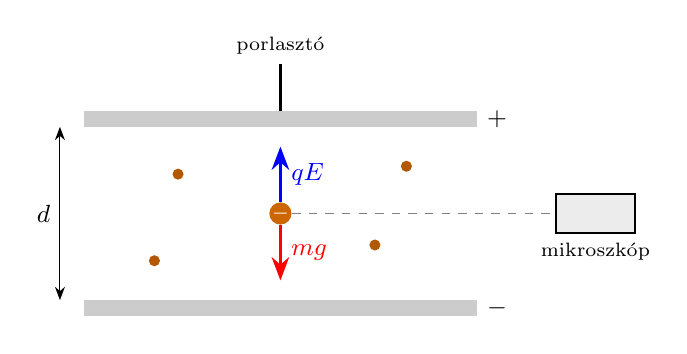
\begin{tikzpicture}[>=Stealth,font=\small]
  \fill[gray!40] (0,2.2) rectangle (5,2.4);
  \fill[gray!40] (0,-0.2) rectangle (5,0);
  \node[right] at (5,2.3) {$+$};
  \node[right] at (5,-0.1) {$-$};
  \draw[<->] (-0.3,0) -- node[left] {$d$} (-0.3,2.2);
  \fill[orange!80!black] (2.5,1.1) circle (4pt);
  \node[font=\scriptsize] at (2.5,1.1) {\color{white}$-$};
  \draw[->,very thick,blue] (2.5,1.25) -- node[right] {$qE$} (2.5,1.95);
  \draw[->,very thick,red] (2.5,0.95) -- node[right] {$mg$} (2.5,0.25);
  \foreach \x/\y in {1.2/1.6,3.7/0.7,4.1/1.7,0.9/0.5} \fill[orange!70!black] (\x,\y) circle (2pt);
  \draw[thick] (2.5,2.4) -- (2.5,3.0);
  \node[above,font=\scriptsize] at (2.5,3.0) {porlasztó};
  \draw[thick,fill=gray!15] (6.0,0.85) rectangle (7.0,1.35);
  \node[below,font=\scriptsize] at (6.5,0.85) {mikroszkóp};
  \draw[dashed,gray] (2.65,1.1) -- (6.0,1.1);
\end{tikzpicture}

\vspace{10pt}
\begin{pelda}
Egy $m = 1{,}6\cdot 10^{-15}$~kg tömegű csepp $d = 5$~mm-es lemeztávolságnál
$U = 490$~V-on lebeg:
\[ q = \frac{mgd}{U} = \frac{1{,}6\cdot 10^{-15}\cdot 9{,}8\cdot 5\cdot 10^{-3}}{490}~\text{C} \]
\[ q = 1{,}6\cdot 10^{-19}~\text{C} = 1\,e \]
A cseppen egyetlen többletelektron ül.
\end{pelda}
\end{minipage}

%====================================================================
\dia{4. Az első modell: Thomson ,,mazsolás puding'' atomja (1904)}

\begin{minipage}[t]{0.60\linewidth}\vspace{0pt}
\begin{itemize}
  \item Az atom semleges, és vannak benne elektronok, tehát kell lennie benne
    \textbf{pozitív töltésnek} is, ami kiegyenlíti őket.
  \item \textbf{Thomson modellje:} az atom egy kb.\ $10^{-10}$~m sugarú gömb, amelyben a
    pozitív töltés és a tömeg \textbf{egyenletesen} oszlik el. Ebbe ágyazódnak be az
    elektronok, mint mazsolák a pudingba.
  \item Megmagyarázta, hogy az atom semleges, és hogy elektronok léphetnek ki belőle
    (ionizáció, katódsugárzás, fotoeffektus).
\end{itemize}
\begin{fontos}
\textbf{A modell jóslata:} ha egy gyors, nehéz, pozitív részecskét (pl.\ $\alpha$-részecskét)
lövünk egy ilyen atomra, az legfeljebb \textbf{nagyon kicsit} térül el, hiszen a pozitív
töltés szétkent, sehol sincs olyan erős tér, ami nagy szögben eltéríthetné. Ezt a jóslatot
lehetett kísérlettel ellenőrizni.
\end{fontos}
\end{minipage}\hfill
\begin{minipage}[t]{0.37\linewidth}\vspace{0pt}\centering
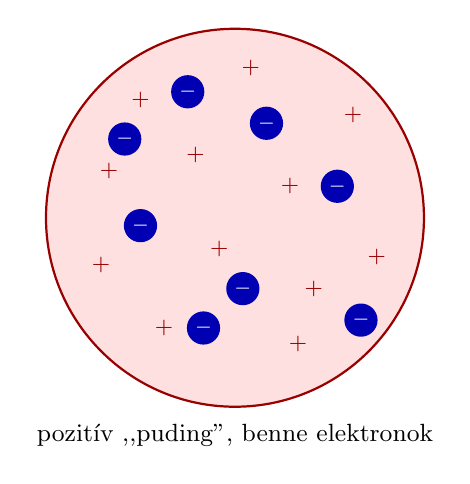
\begin{tikzpicture}[font=\small]
  \fill[red!12] (0,0) circle (2.4);
  \draw[thick,red!60!black] (0,0) circle (2.4);
  \foreach \x/\y in {-1.6/0.6,-0.9/-1.4,-1.2/1.5,0.2/1.9,1.5/1.3,1.8/-0.5,0.8/-1.6,-0.2/-0.4,
                     0.7/0.4,-1.7/-0.6,1.0/-0.9,-0.5/0.8}
    \node[red!60!black,font=\footnotesize] at (\x,\y) {$+$};
  \foreach \x/\y in {-1.2/-0.1,-0.4/-1.4,0.4/1.2,1.3/0.4,-0.6/1.6,0.1/-0.9,1.6/-1.3,-1.4/1.0}{
    \fill[blue!70!black] (\x,\y) circle (6pt);
    \node[white,font=\scriptsize] at (\x,\y) {$-$};}
  \node[below] at (0,-2.5) {pozitív ,,puding'', benne elektronok};
\end{tikzpicture}
\end{minipage}

%====================================================================
\dia{5. A döntő kísérlet: $\alpha$-részecskék szórása aranyfólián (1909--1911)}

\begin{minipage}[t]{0.50\linewidth}\vspace{0pt}
\begin{itemize}
  \item \textbf{Geiger és Marsden} Rutherford irányításával radioaktív forrásból
    kilépő $\alpha$-részecskékkel (pozitív, nehéz, gyors részecskék) lőtték egy nagyon
    vékony (kb.\ $1000$ atomnyi) aranyfóliát, \textbf{vákuumban}.
  \item A szórt részecskéket egy cink-szulfid ernyő villanásai jelezték, ezeket
    mikroszkóppal, egyenként számolták meg, minden irányban.
  \item \textbf{Eredmények:}
    \begin{itemize}
      \item a részecskék \textbf{túlnyomó többsége eltérülés nélkül} áthalad;
      \item néhány \textbf{nagy szögben} eltérül;
      \item kb.\ minden $8000$.\ \textbf{visszapattan}!
    \end{itemize}
\end{itemize}
{\small\emph{Rutherford:} ,,Olyan hihetetlen volt, mintha egy ágyúgolyót lőttünk volna egy
selyempapírra, és az visszapattant volna.''}
\end{minipage}\hfill
\begin{minipage}[t]{0.47\linewidth}\vspace{0pt}\centering
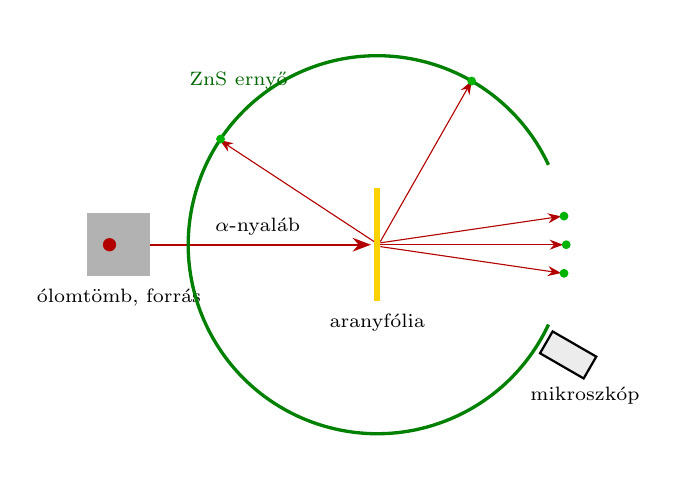
\begin{tikzpicture}[scale=0.8,>=Stealth,font=\small]
  % forrás
  \fill[gray!60] (-4.6,-0.5) rectangle (-3.6,0.5);
  \fill[red!70!black] (-4.25,0) circle (3pt);
  \node[below,font=\scriptsize] at (-4.1,-0.55) {ólomtömb, forrás};
  \draw[->,thick,red!70!black] (-3.6,0) -- (-0.1,0);
  \node[above,font=\scriptsize] at (-1.9,0) {$\alpha$-nyaláb};
  % fólia
  \fill[yellow!70!orange] (-0.05,-0.9) rectangle (0.05,0.9);
  \node[below,font=\scriptsize] at (0,-0.95) {aranyfólia};
  % ernyő
  \draw[very thick,green!50!black] (0,0) ++(25:3.0) arc (25:335:3.0);
  \node[green!40!black,font=\scriptsize] at (-2.2,2.6) {ZnS ernyő};
  % szórt utak
  \draw[->,red!70!black] (0.05,0) -- (2.95,0);
  \draw[->,red!70!black] (0.05,0.03) -- (2.92,0.45);
  \draw[->,red!70!black] (0.05,-0.03) -- (2.92,-0.45);
  \draw[->,red!70!black] (0.05,0.05) -- (1.5,2.6);
  \draw[->,red!70!black] (-0.05,0.05) -- (-2.5,1.66);
  \foreach \a in {0,8.7,-8.7,60,146} \fill[green!70!black] (\a:3.0) circle (2pt);
  % mikroszkóp
  \draw[thick,fill=gray!15,rotate around={-30:(0,0)}] (3.1,-0.2) rectangle (3.9,0.2);
  \node[font=\scriptsize] at (3.3,-2.4) {mikroszkóp};
\end{tikzpicture}

\vspace{4pt}
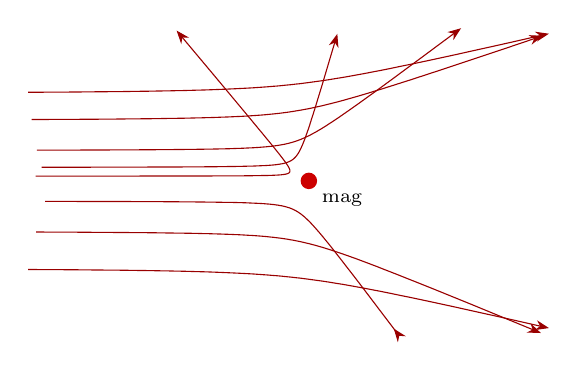
\begin{tikzpicture}[scale=0.85,>=Stealth,font=\small]
  \fill[red!80!black] (0,0) circle (3.5pt);
  \node[below right,font=\scriptsize] at (0.05,-0.05) {mag};
  \draw[->,red!60!black] plot[smooth] coordinates {(-4.193,1.324) (-3.810,1.326) (-3.487,1.328) (-3.209,1.331) (-2.967,1.333) (-2.755,1.335) (-2.567,1.338) (-2.399,1.340) (-2.247,1.343) (-2.109,1.345) (-1.983,1.348) (-1.868,1.350) (-1.761,1.353) (-1.662,1.356) (-1.570,1.358) (-1.483,1.361) (-1.402,1.364) (-1.325,1.367) (-1.253,1.370) (-1.184,1.373) (-1.118,1.376) (-1.056,1.379) (-0.996,1.382) (-0.938,1.385) (-0.882,1.388) (-0.828,1.391) (-0.776,1.395) (-0.726,1.398) (-0.677,1.402) (-0.629,1.405) (-0.582,1.409) (-0.536,1.413) (-0.490,1.416) (-0.446,1.420) (-0.402,1.424) (-0.359,1.429) (-0.316,1.433) (-0.273,1.437) (-0.231,1.442) (-0.188,1.447) (-0.146,1.451) (-0.104,1.456) (-0.062,1.462) (-0.019,1.467) (0.024,1.473) (0.067,1.479) (0.111,1.485) (0.155,1.491) (0.200,1.497) (0.245,1.504) (0.292,1.511) (0.340,1.519) (0.388,1.527) (0.438,1.535) (0.490,1.543) (0.543,1.552) (0.598,1.562) (0.655,1.572) (0.714,1.583) (0.776,1.594) (0.840,1.606) (0.908,1.619) (0.979,1.633) (1.055,1.647) (1.134,1.663) (1.219,1.680) (1.309,1.699) (1.406,1.719) (1.511,1.740) (1.624,1.764) (1.747,1.790) (1.882,1.819) (2.030,1.851) (2.195,1.887) (2.379,1.928) (2.586,1.974) (2.821,2.026) (3.092,2.087) (3.408,2.159) (3.587,2.199)};
  \draw[->,red!60!black] plot[smooth] coordinates {(-4.141,0.917) (-3.660,0.919) (-3.276,0.921) (-2.962,0.923) (-2.700,0.926) (-2.477,0.928) (-2.286,0.930) (-2.119,0.933) (-1.972,0.935) (-1.841,0.937) (-1.725,0.940) (-1.619,0.942) (-1.523,0.945) (-1.436,0.947) (-1.355,0.950) (-1.281,0.953) (-1.211,0.955) (-1.147,0.958) (-1.087,0.961) (-1.030,0.963) (-0.976,0.966) (-0.926,0.969) (-0.878,0.972) (-0.832,0.975) (-0.788,0.978) (-0.746,0.981) (-0.706,0.984) (-0.667,0.987) (-0.629,0.991) (-0.593,0.994) (-0.557,0.998) (-0.523,1.001) (-0.489,1.005) (-0.457,1.008) (-0.424,1.012) (-0.393,1.016) (-0.362,1.020) (-0.331,1.024) (-0.301,1.028) (-0.271,1.033) (-0.241,1.037) (-0.212,1.042) (-0.182,1.047) (-0.153,1.052) (-0.123,1.057) (-0.094,1.062) (-0.064,1.068) (-0.034,1.073) (-0.004,1.079) (0.027,1.085) (0.058,1.092) (0.089,1.099) (0.121,1.106) (0.153,1.113) (0.187,1.120) (0.221,1.128) (0.256,1.137) (0.292,1.146) (0.329,1.155) (0.368,1.165) (0.408,1.175) (0.449,1.186) (0.493,1.198) (0.538,1.210) (0.586,1.224) (0.636,1.238) (0.689,1.253) (0.745,1.269) (0.805,1.287) (0.869,1.306) (0.937,1.327) (1.011,1.350) (1.092,1.374) (1.179,1.402) (1.275,1.432) (1.381,1.466) (1.498,1.503) (1.630,1.546) (1.779,1.595) (1.948,1.650) (2.144,1.715) (2.373,1.791) (2.644,1.882) (2.973,1.992) (3.378,2.129) (3.495,2.168)};
  \draw[->,red!60!black] plot[smooth] coordinates {(-4.062,0.459) (-3.331,0.461) (-2.824,0.463) (-2.450,0.465) (-2.164,0.467) (-1.937,0.469) (-1.753,0.471) (-1.600,0.473) (-1.471,0.475) (-1.361,0.477) (-1.265,0.479) (-1.181,0.481) (-1.106,0.484) (-1.040,0.486) (-0.980,0.488) (-0.926,0.491) (-0.877,0.493) (-0.832,0.495) (-0.791,0.498) (-0.752,0.500) (-0.717,0.503) (-0.683,0.506) (-0.652,0.508) (-0.623,0.511) (-0.595,0.514) (-0.569,0.516) (-0.544,0.519) (-0.521,0.522) (-0.498,0.525) (-0.477,0.528) (-0.456,0.531) (-0.436,0.535) (-0.417,0.538) (-0.398,0.541) (-0.380,0.545) (-0.362,0.548) (-0.345,0.552) (-0.329,0.556) (-0.312,0.559) (-0.296,0.563) (-0.281,0.568) (-0.265,0.572) (-0.250,0.576) (-0.235,0.580) (-0.220,0.585) (-0.205,0.590) (-0.190,0.595) (-0.175,0.600) (-0.161,0.605) (-0.146,0.611) (-0.131,0.616) (-0.116,0.622) (-0.101,0.629) (-0.086,0.635) (-0.070,0.642) (-0.055,0.649) (-0.039,0.656) (-0.023,0.664) (-0.006,0.672) (0.011,0.680) (0.028,0.689) (0.046,0.699) (0.064,0.709) (0.083,0.719) (0.103,0.730) (0.124,0.742) (0.145,0.755) (0.168,0.768) (0.192,0.782) (0.217,0.798) (0.243,0.814) (0.271,0.832) (0.301,0.852) (0.334,0.873) (0.368,0.896) (0.406,0.921) (0.447,0.948) (0.491,0.979) (0.540,1.013) (0.595,1.051) (0.656,1.094) (0.724,1.142) (0.802,1.198) (0.892,1.263) (0.997,1.338) (1.120,1.428) (1.269,1.537) (1.451,1.672) (1.682,1.842) (1.981,2.064) (2.274,2.281)};
  \draw[->,red!60!black] plot[smooth] coordinates {(-3.994,0.204) (-2.948,0.205) (-2.342,0.207) (-1.946,0.208) (-1.668,0.210) (-1.461,0.211) (-1.301,0.213) (-1.174,0.215) (-1.070,0.216) (-0.984,0.218) (-0.911,0.220) (-0.849,0.221) (-0.795,0.223) (-0.748,0.225) (-0.706,0.227) (-0.669,0.228) (-0.635,0.230) (-0.605,0.232) (-0.578,0.234) (-0.554,0.236) (-0.531,0.238) (-0.510,0.240) (-0.491,0.242) (-0.473,0.245) (-0.456,0.247) (-0.441,0.249) (-0.426,0.252) (-0.413,0.254) (-0.400,0.256) (-0.388,0.259) (-0.376,0.261) (-0.365,0.264) (-0.355,0.267) (-0.345,0.270) (-0.336,0.272) (-0.327,0.275) (-0.318,0.278) (-0.310,0.282) (-0.302,0.285) (-0.295,0.288) (-0.287,0.292) (-0.280,0.295) (-0.273,0.299) (-0.267,0.302) (-0.260,0.306) (-0.254,0.310) (-0.248,0.315) (-0.241,0.319) (-0.236,0.323) (-0.230,0.328) (-0.224,0.333) (-0.219,0.338) (-0.213,0.343) (-0.208,0.349) (-0.202,0.354) (-0.197,0.360) (-0.191,0.367) (-0.186,0.373) (-0.181,0.380) (-0.176,0.387) (-0.170,0.395) (-0.165,0.403) (-0.159,0.411) (-0.154,0.420) (-0.148,0.429) (-0.143,0.439) (-0.137,0.450) (-0.131,0.461) (-0.125,0.473) (-0.119,0.486) (-0.113,0.500) (-0.106,0.515) (-0.099,0.530) (-0.092,0.548) (-0.084,0.566) (-0.076,0.587) (-0.067,0.609) (-0.058,0.633) (-0.048,0.660) (-0.038,0.690) (-0.026,0.723) (-0.013,0.760) (0.001,0.802) (0.017,0.850) (0.034,0.905) (0.055,0.969) (0.079,1.045) (0.107,1.135) (0.140,1.244) (0.182,1.380) (0.234,1.554) (0.302,1.783) (0.396,2.098) (0.425,2.197)};
  \draw[->,red!60!black] plot[smooth] coordinates {(-4.084,0.071) (-2.749,0.072) (-2.081,0.073) (-1.681,0.073) (-1.414,0.074) (-1.224,0.075) (-1.081,0.076) (-0.971,0.076) (-0.882,0.077) (-0.810,0.078) (-0.750,0.079) (-0.699,0.080) (-0.656,0.081) (-0.618,0.081) (-0.586,0.082) (-0.557,0.083) (-0.531,0.084) (-0.509,0.085) (-0.488,0.086) (-0.470,0.087) (-0.454,0.088) (-0.439,0.089) (-0.425,0.090) (-0.412,0.091) (-0.401,0.093) (-0.390,0.094) (-0.381,0.095) (-0.372,0.096) (-0.364,0.098) (-0.356,0.099) (-0.349,0.100) (-0.343,0.102) (-0.337,0.103) (-0.331,0.104) (-0.326,0.106) (-0.321,0.108) (-0.317,0.109) (-0.313,0.111) (-0.309,0.113) (-0.306,0.114) (-0.302,0.116) (-0.300,0.118) (-0.297,0.120) (-0.294,0.122) (-0.292,0.124) (-0.290,0.126) (-0.289,0.129) (-0.287,0.131) (-0.286,0.133) (-0.285,0.136) (-0.284,0.139) (-0.283,0.141) (-0.283,0.144) (-0.283,0.147) (-0.283,0.150) (-0.283,0.154) (-0.283,0.157) (-0.284,0.161) (-0.285,0.165) (-0.286,0.169) (-0.287,0.173) (-0.289,0.177) (-0.291,0.182) (-0.293,0.187) (-0.295,0.192) (-0.298,0.197) (-0.301,0.203) (-0.305,0.209) (-0.308,0.216) (-0.313,0.223) (-0.317,0.231) (-0.323,0.239) (-0.329,0.248) (-0.335,0.257) (-0.342,0.268) (-0.350,0.279) (-0.359,0.291) (-0.369,0.304) (-0.380,0.319) (-0.392,0.335) (-0.406,0.353) (-0.421,0.373) (-0.439,0.396) (-0.460,0.422) (-0.483,0.451) (-0.510,0.485) (-0.542,0.524) (-0.580,0.571) (-0.626,0.626) (-0.682,0.695) (-0.753,0.780) (-0.844,0.890) (-0.965,1.036) (-1.136,1.241) (-1.392,1.548) (-1.821,2.060) (-1.976,2.246)};
  \draw[->,red!60!black] plot[smooth] coordinates {(-3.940,-0.306) (-3.077,-0.308) (-2.528,-0.309) (-2.147,-0.311) (-1.868,-0.313) (-1.653,-0.315) (-1.483,-0.317) (-1.346,-0.319) (-1.231,-0.321) (-1.135,-0.322) (-1.053,-0.324) (-0.982,-0.326) (-0.919,-0.328) (-0.864,-0.331) (-0.815,-0.333) (-0.771,-0.335) (-0.731,-0.337) (-0.695,-0.339) (-0.662,-0.341) (-0.632,-0.344) (-0.604,-0.346) (-0.578,-0.348) (-0.554,-0.351) (-0.531,-0.353) (-0.510,-0.356) (-0.491,-0.359) (-0.472,-0.361) (-0.454,-0.364) (-0.438,-0.367) (-0.422,-0.370) (-0.406,-0.372) (-0.392,-0.375) (-0.378,-0.378) (-0.365,-0.382) (-0.352,-0.385) (-0.339,-0.388) (-0.327,-0.392) (-0.316,-0.395) (-0.304,-0.399) (-0.293,-0.402) (-0.282,-0.406) (-0.272,-0.410) (-0.262,-0.414) (-0.251,-0.418) (-0.241,-0.423) (-0.232,-0.427) (-0.222,-0.432) (-0.212,-0.437) (-0.203,-0.442) (-0.193,-0.447) (-0.184,-0.452) (-0.174,-0.458) (-0.165,-0.464) (-0.155,-0.470) (-0.146,-0.476) (-0.136,-0.483) (-0.127,-0.489) (-0.117,-0.497) (-0.107,-0.504) (-0.097,-0.512) (-0.087,-0.521) (-0.076,-0.529) (-0.065,-0.539) (-0.054,-0.549) (-0.043,-0.559) (-0.031,-0.570) (-0.019,-0.582) (-0.006,-0.594) (0.008,-0.608) (0.022,-0.622) (0.036,-0.637) (0.052,-0.654) (0.068,-0.671) (0.085,-0.691) (0.104,-0.712) (0.124,-0.735) (0.146,-0.760) (0.169,-0.787) (0.195,-0.818) (0.223,-0.852) (0.254,-0.890) (0.289,-0.932) (0.328,-0.981) (0.372,-1.037) (0.423,-1.102) (0.482,-1.177) (0.552,-1.268) (0.637,-1.377) (0.740,-1.511) (0.870,-1.682) (1.039,-1.905) (1.269,-2.208) (1.269,-2.208)};
  \draw[->,red!60!black] plot[smooth] coordinates {(-4.074,-0.764) (-3.546,-0.766) (-3.136,-0.769) (-2.809,-0.771) (-2.541,-0.773) (-2.318,-0.775) (-2.129,-0.778) (-1.966,-0.780) (-1.824,-0.782) (-1.699,-0.784) (-1.588,-0.787) (-1.488,-0.789) (-1.399,-0.792) (-1.317,-0.794) (-1.243,-0.797) (-1.175,-0.799) (-1.112,-0.802) (-1.053,-0.804) (-0.998,-0.807) (-0.947,-0.810) (-0.899,-0.813) (-0.854,-0.815) (-0.811,-0.818) (-0.771,-0.821) (-0.732,-0.824) (-0.695,-0.827) (-0.659,-0.830) (-0.625,-0.833) (-0.593,-0.837) (-0.561,-0.840) (-0.530,-0.843) (-0.500,-0.847) (-0.472,-0.850) (-0.443,-0.854) (-0.416,-0.857) (-0.389,-0.861) (-0.362,-0.865) (-0.336,-0.869) (-0.310,-0.873) (-0.285,-0.878) (-0.260,-0.882) (-0.235,-0.886) (-0.210,-0.891) (-0.186,-0.896) (-0.161,-0.901) (-0.136,-0.906) (-0.112,-0.911) (-0.087,-0.917) (-0.062,-0.923) (-0.037,-0.929) (-0.011,-0.935) (0.015,-0.941) (0.041,-0.948) (0.067,-0.955) (0.094,-0.962) (0.122,-0.970) (0.151,-0.978) (0.180,-0.987) (0.210,-0.995) (0.241,-1.005) (0.273,-1.015) (0.306,-1.025) (0.341,-1.036) (0.377,-1.048) (0.415,-1.061) (0.454,-1.074) (0.496,-1.088) (0.540,-1.104) (0.587,-1.120) (0.636,-1.138) (0.690,-1.157) (0.747,-1.178) (0.808,-1.201) (0.875,-1.226) (0.948,-1.254) (1.028,-1.284) (1.115,-1.319) (1.213,-1.357) (1.323,-1.400) (1.446,-1.449) (1.587,-1.505) (1.750,-1.570) (1.941,-1.647) (2.167,-1.739) (2.440,-1.850) (2.777,-1.989) (3.206,-2.165) (3.467,-2.273)};
  \draw[->,red!60!black] plot[smooth] coordinates {(-4.193,-1.324) (-3.810,-1.326) (-3.487,-1.328) (-3.209,-1.331) (-2.967,-1.333) (-2.755,-1.335) (-2.567,-1.338) (-2.399,-1.340) (-2.247,-1.343) (-2.109,-1.345) (-1.983,-1.348) (-1.868,-1.350) (-1.761,-1.353) (-1.662,-1.356) (-1.570,-1.358) (-1.483,-1.361) (-1.402,-1.364) (-1.325,-1.367) (-1.253,-1.370) (-1.184,-1.373) (-1.118,-1.376) (-1.056,-1.379) (-0.996,-1.382) (-0.938,-1.385) (-0.882,-1.388) (-0.828,-1.391) (-0.776,-1.395) (-0.726,-1.398) (-0.677,-1.402) (-0.629,-1.405) (-0.582,-1.409) (-0.536,-1.413) (-0.490,-1.416) (-0.446,-1.420) (-0.402,-1.424) (-0.359,-1.429) (-0.316,-1.433) (-0.273,-1.437) (-0.231,-1.442) (-0.188,-1.447) (-0.146,-1.451) (-0.104,-1.456) (-0.062,-1.462) (-0.019,-1.467) (0.024,-1.473) (0.067,-1.479) (0.111,-1.485) (0.155,-1.491) (0.200,-1.497) (0.245,-1.504) (0.292,-1.511) (0.340,-1.519) (0.388,-1.527) (0.438,-1.535) (0.490,-1.543) (0.543,-1.552) (0.598,-1.562) (0.655,-1.572) (0.714,-1.583) (0.776,-1.594) (0.840,-1.606) (0.908,-1.619) (0.979,-1.633) (1.055,-1.647) (1.134,-1.663) (1.219,-1.680) (1.309,-1.699) (1.406,-1.719) (1.511,-1.740) (1.624,-1.764) (1.747,-1.790) (1.882,-1.819) (2.030,-1.851) (2.195,-1.887) (2.379,-1.928) (2.586,-1.974) (2.821,-2.026) (3.092,-2.087) (3.408,-2.159) (3.587,-2.199)};
\end{tikzpicture}\\
{\scriptsize minél közelebb halad el a mag mellett, annál jobban eltérül}
\end{minipage}

%====================================================================
\dia{6. A Rutherford-modell (1911) és a problémái}

\begin{minipage}[t]{0.60\linewidth}\vspace{0pt}
\textbf{Következtetés a szórásból:} a pozitív töltés és a tömeg $99{,}9\%$-a egy
\textbf{parányi atommagban} összpontosul. Csak ennek a közelében elég erős az
elektromos tér a nagy eltérítéshez. A mag sugara $10^{-15}$--$10^{-14}$~m, az atomé
$10^{-10}$~m.
\begin{itemize}
  \item \textbf{Bolygómodell:} az elektronok úgy keringenek a mag körül, mint a bolygók a
    Nap körül. A centripetális erőt a Coulomb-vonzás adja. Az atom szinte teljesen
    \textbf{üres}.
\end{itemize}

\begin{pelda}[title=Arányok]
$\dfrac{r_\text{atom}}{r_\text{mag}} \approx \dfrac{10^{-10}~\text{m}}{10^{-15}~\text{m}} = 10^5$.
Ha az atommag egy $5$~mm-es borsószem lenne, az atom egy $500$~m átmérőjű gömb, a
legközelebbi elektronok kb.\ $250$~m-re lennének tőle.
\end{pelda}

\textbf{Két súlyos probléma} a klasszikus fizika szerint:
\begin{enumerate}[label=\textbf{\arabic*.},leftmargin=1.6em,itemsep=2pt,topsep=2pt]
  \item \textbf{Instabilitás:} a körpályán keringő elektron gyorsul. A gyorsuló töltés
    elektromágneses hullámot sugároz, ezért energiát veszít, és kb.\ $10^{-11}$~s alatt
    spirálpályán \textbf{a magba zuhanna}. Az atomok mégis stabilak.
  \item \textbf{Folytonos színkép:} a spirálozó elektron keringési frekvenciája folyamatosan
    változna, így minden hullámhosszon sugározna. Az atomok viszont \textbf{vonalas}
    színképet adnak (következő dia).
\end{enumerate}
\end{minipage}\hfill
\begin{minipage}[t]{0.37\linewidth}\vspace{0pt}\centering
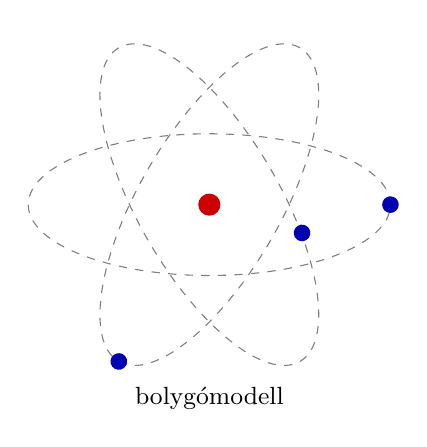
\begin{tikzpicture}[>=Stealth,font=\small]
  \draw[gray,dashed] (0,0) ellipse (2.3 and 0.9);
  \draw[gray,dashed,rotate=60] (0,0) ellipse (2.3 and 0.9);
  \draw[gray,dashed,rotate=-60] (0,0) ellipse (2.3 and 0.9);
  \fill[red!80!black] (0,0) circle (4pt);
  \foreach \a/\r in {20/{2.3 and 0.9}}{}
  \fill[blue!70!black] (2.3,0) circle (3pt);
  \fill[blue!70!black,rotate=60] (-2.3,0) circle (3pt);
  \fill[blue!70!black,rotate=-60] (0.9,0.84) circle (3pt);
  \node[below] at (0,-2.2) {bolygómodell};
\end{tikzpicture}

\vspace{14pt}
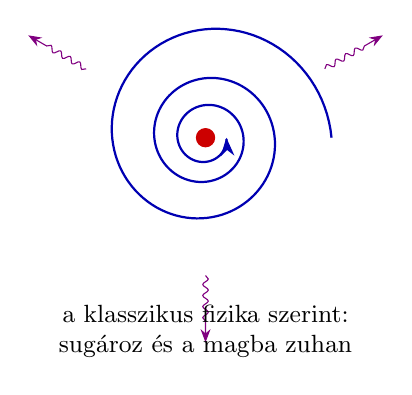
\begin{tikzpicture}[>=Stealth,font=\small]
  \fill[red!80!black] (0,0) circle (3.5pt);
  \draw[thick,blue!70!black,domain=0:1080,samples=300,->]
    plot ({1.6*exp(-\x/600)*cos(\x)},{1.6*exp(-\x/600)*sin(\x)});
  \foreach \a in {30,150,270}
    \draw[->,violet,decorate,decoration={snake,amplitude=1pt,segment length=4pt,post length=2mm}]
      (\a:1.75) -- (\a:2.6);
  \node[below,align=center] at (0,-2.0) {a klasszikus fizika szerint:\\sugároz és a magba zuhan};
\end{tikzpicture}
\end{minipage}

%====================================================================
\dia{7. Vonalas színképek: az atomok ujjlenyomata}

\begin{itemize}
  \item \textbf{Kirchhoff és Bunsen (1859):} a hevített gázok (pl.\ lángba szórt sók, gázkisülési
    csövek) fénye prizmán vagy rácson felbontva nem folytonos, hanem néhány éles,
    \textbf{színes vonalból} áll. Minden elem vonalai mások: ez az elem
    \textbf{ujjlenyomata} (színképelemzés).
  \item \textbf{Elnyelési színkép:} ha folytonos színképű fehér fény hideg gázon halad át,
    a gáz \emph{ugyanazokon} a hullámhosszakon nyel el, amelyeken izzó állapotban
    sugároz. A Nap színképének sötét vonalai (Fraunhofer-vonalak) így árulják el a
    Nap légkörének összetételét: a héliumot 1868-ban a Napban fedezték fel, csak később
    a Földön.
\end{itemize}

\vspace{2pt}
\begin{center}
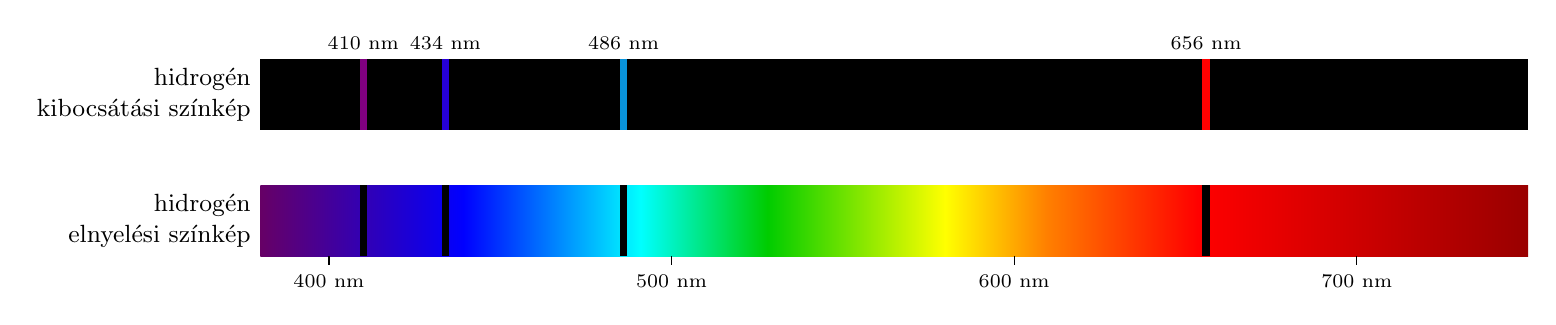
\begin{tikzpicture}[x=1.15cm,font=\small]
  % kibocsátási színkép
  \fill[black] (0,1.6) rectangle (14,2.5);
  \foreach \l/\c in {410/violet,434/blue!70!violet,486/cyan!80!blue,656/red}{
    \pgfmathsetmacro{\xx}{(\l-380)/370*14}
    \fill[\c] (\xx-0.04,1.6) rectangle (\xx+0.04,2.5);
    \node[above,font=\scriptsize] at (\xx,2.5) {\l~nm};}
  \node[left,align=right] at (0,2.05) {hidrogén\\kibocsátási színkép};
  % elnyelési színkép
  \shade[shading=lathato] (0,0) rectangle (14,0.9);
  \foreach \l in {410,434,486,656}{
    \pgfmathsetmacro{\xx}{(\l-380)/370*14}
    \fill[black] (\xx-0.04,0) rectangle (\xx+0.04,0.9);}
  \node[left,align=right] at (0,0.45) {hidrogén\\elnyelési színkép};
  \foreach \l in {400,500,600,700}{
    \pgfmathsetmacro{\xx}{(\l-380)/370*14}
    \draw (\xx,0) -- (\xx,-0.12) node[below,font=\scriptsize] {\l~nm};}
\end{tikzpicture}
\end{center}

\begin{fontos}
\textbf{Balmer (1885)} a hidrogén látható vonalaira tapasztalati képletet talált, de
\emph{senki sem tudta, miért} ilyenek. A Rutherford-modell szerint egyáltalán nem is
lehetnének vonalak.
\end{fontos}

%====================================================================
\dia{8. A Bohr-modell (1913): kvantált pályák}

\begin{minipage}[t]{0.55\linewidth}\vspace{0pt}
Bohr megtartotta a Rutherford-modellt, de Planck kvantumgondolatát alkalmazta rá.
\textbf{Bohr posztulátumai:}
\begin{enumerate}[label=\textbf{\arabic*.},leftmargin=1.6em,itemsep=3pt,topsep=2pt]
  \item Az elektron csak bizonyos megengedett (\textbf{stacionárius}) pályákon keringhet, és
    ezeken \textbf{nem sugároz}. Az atom ezért stabil.
  \item Az atom csak akkor bocsát ki (vagy nyel el) fényt, ha az elektron egyik pályáról
    a másikra \textbf{ugrik}. A foton energiája a két szint energiájának különbsége:
    \[ hf = E_\text{felső} - E_\text{alsó} \]
  \item A megengedett pályákon az elektron impulzusmomentuma $\dfrac{h}{2\pi}$ egész
    számú többszöröse: $\;mvr = n\dfrac{h}{2\pi}$, $\;n = 1, 2, 3, \dots$
\end{enumerate}
\begin{fontos}
A hidrogénatom energiaszintjei és pályasugarai:
\[ E_n = -\frac{13{,}6~\text{eV}}{n^2}, \qquad r_n = n^2\cdot 0{,}053~\text{nm} \]
A negatív előjel azt jelenti, hogy az elektron \textbf{kötött}: $13{,}6$~eV kell ahhoz,
hogy alapállapotból kiszakítsuk (\textbf{ionizációs energia}).
\end{fontos}
\end{minipage}\hfill
\begin{minipage}[t]{0.42\linewidth}\vspace{0pt}\centering
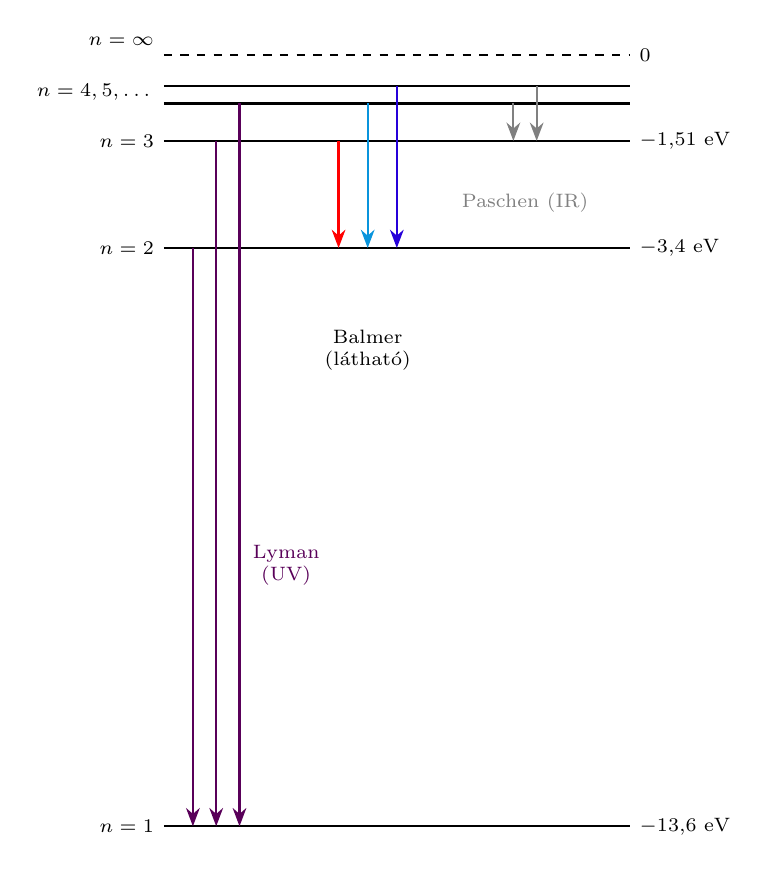
\begin{tikzpicture}[x=0.74cm,y=0.72cm,>=Stealth,font=\small]
  \foreach \n in {1,2,3,4,5}{
    \pgfmathsetmacro{\E}{-13.6/(\n*\n)}
    \draw[thick] (0,\E) -- (8,\E);}
  \foreach \n in {1,2,3}{
    \pgfmathsetmacro{\E}{-13.6/(\n*\n)}
    \node[left,font=\scriptsize] at (0,\E) {$n=\n$};}
  \node[left,font=\scriptsize] at (0,-0.65) {$n=4,5,\dots$};
  \draw[thick,dashed] (0,0) -- (8,0);
  \node[left,font=\scriptsize] at (0,0.25) {$n=\infty$};
  \node[right,font=\scriptsize] at (8,-13.6) {$-13{,}6$~eV};
  \node[right,font=\scriptsize] at (8,-3.4) {$-3{,}4$~eV};
  \node[right,font=\scriptsize] at (8,-1.51) {$-1{,}51$~eV};
  \node[right,font=\scriptsize] at (8,0) {$0$};
  % Lyman
  \foreach \n/\x in {2/0.5,3/0.9,4/1.3}{
    \pgfmathsetmacro{\E}{-13.6/(\n*\n)}
    \draw[->,violet!70!black,thick] (\x,\E) -- (\x,-13.6);}
  \node[violet!70!black,font=\scriptsize,align=center,fill=white,inner sep=1pt] at (2.1,-9) {Lyman\\(UV)};
  % Balmer
  \foreach \n/\x/\c in {3/3.0/red,4/3.5/cyan!80!blue,5/4.0/blue!70!violet}{
    \pgfmathsetmacro{\E}{-13.6/(\n*\n)}
    \draw[->,\c,thick] (\x,\E) -- (\x,-3.4);}
  \node[font=\scriptsize,align=center] at (3.5,-5.2) {Balmer\\(látható)};
  % Paschen
  \foreach \n/\x in {4/6.0,5/6.4}{
    \pgfmathsetmacro{\E}{-13.6/(\n*\n)}
    \draw[->,gray,thick] (\x,\E) -- (\x,-1.51);}
  \node[gray,font=\scriptsize,align=center] at (6.2,-2.6) {Paschen (IR)};
\end{tikzpicture}
\end{minipage}

%====================================================================
\dia{9. Kidolgozott példa: a hidrogén színképe a Bohr-modellből}

\begin{pelda}
\textbf{Az $n=3 \to n=2$ átmenet:}
$\;hf = E_3 - E_2 = -\dfrac{13{,}6}{9} + \dfrac{13{,}6}{4} = 13{,}6\left(\dfrac14 - \dfrac19\right)~\text{eV}
  \approx 1{,}89~\text{eV}$,\quad
$\lambda = \dfrac{1240~\text{eV}\cdot\text{nm}}{1{,}89~\text{eV}} \approx 656~\text{nm}$
\quad (vörös).

\medskip
\textbf{Az $n=4 \to n=2$ átmenet:}
$\;hf = 13{,}6\left(\dfrac14 - \dfrac1{16}\right)~\text{eV} = 2{,}55~\text{eV}$,\quad
$\lambda \approx 486~\text{nm}$ \quad (kékeszöld).

\medskip
\textbf{Az $n=2 \to n=1$ átmenet:}
$\;hf = 13{,}6\left(1 - \dfrac14\right)~\text{eV} = 10{,}2~\text{eV}$,\quad
$\lambda \approx 122~\text{nm}$ \quad (ultraibolya: szemmel nem látható).
\end{pelda}

\begin{itemize}
  \item A kiszámolt hullámhosszak \textbf{pontosan egyeznek} a hidrogén mért
    színképvonalaival (656, 486, 434, 410~nm). Ez volt a Bohr-modell legnagyobb sikere.
  \item \textbf{Elnyelés:} alapállapotú hidrogén csak olyan fotont nyelhet el, amelynek
    energiája pontosan egy szintkülönbséggel egyezik (legalább $10{,}2$~eV). A látható
    fény fotonjai ($1{,}6$--$3{,}3$~eV) ehhez kevesek, ezért a hidrogéngáz
    \textbf{átlátszó}.
  \item \textbf{Ionizáció:} $13{,}6$~eV-nál nagyobb energiájú foton bármekkora lehet: a
    maradék az elektron mozgási energiája lesz (mint a fotoeffektusnál).
\end{itemize}

%====================================================================
\dia{10. Franck--Hertz-kísérlet (1914): az energiaszintek közvetlen bizonyítéka}

\begin{minipage}[t]{0.52\linewidth}\vspace{0pt}
\begin{itemize}
  \item Elektronokat \textbf{gyorsítottak higanygőzzel} töltött csőben, és mérték, hány jut
    el a gyűjtőelektródára (anódáram), a gyorsítófeszültség függvényében.
  \item Az áram nőtt, majd \textbf{$4{,}9$~V-nál hirtelen leesett}, aztán újra nőtt, és
    $9{,}8$~V-nál, $14{,}7$~V-nál ismét leesett.
  \item \textbf{Magyarázat:} a higanyatom csak \textbf{pontosan $4{,}9$~eV} energiát tud
    felvenni (ennyi az első gerjesztett szint). Kisebb energiájú elektron rugalmasan
    pattan róla, nem veszít energiát. $4{,}9$~eV-nál az elektronok ütközéskor elveszítik
    az energiájukat, és nem jutnak el az anódig. $9{,}8$~V-nál egy elektron
    \emph{kétszer} tud gerjeszteni, és így tovább.
  \item A gerjesztett higanyatomok visszaugráskor
    $\lambda = \dfrac{1240}{4{,}9}~\text{nm} \approx 253~\text{nm}$-es UV fényt bocsátanak
    ki. Ezt valóban megmérték.
\end{itemize}
\begin{fontos}
Ez \textbf{ütközéssel}, a színképektől függetlenül igazolta, hogy az atom energiája
\textbf{csak meghatározott értékeket} vehet fel (Nobel-díj, 1925).
\end{fontos}
\end{minipage}\hfill
\begin{minipage}[t]{0.45\linewidth}\vspace{0pt}\centering
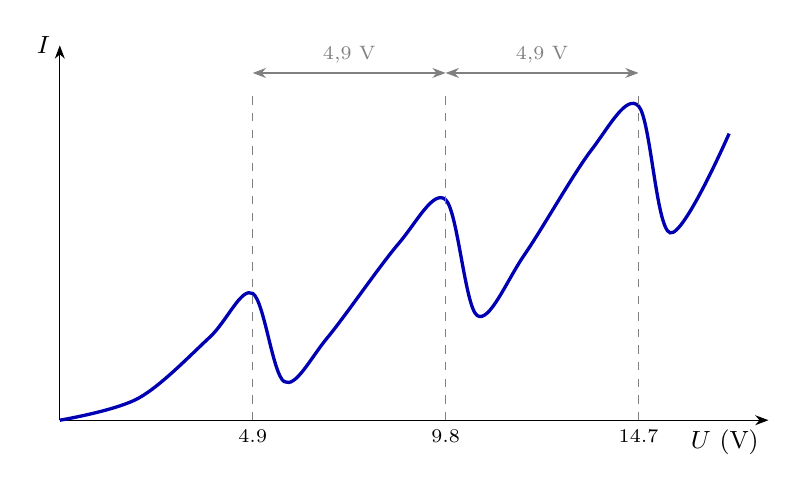
\begin{tikzpicture}[x=0.5cm,y=1.4cm,>=Stealth,font=\small]
  \draw[->] (0,0) -- (18,0) node[below left] {$U$ (V)};
  \draw[->] (0,0) -- (0,3.4) node[left] {$I$};
  \draw[very thick,blue!70!black] plot[smooth,tension=0.55] coordinates {
    (0,0) (2,0.2) (3.8,0.75) (4.9,1.15) (5.7,0.35) (6.8,0.75) (8.6,1.6) (9.8,2.0)
    (10.6,0.95) (11.8,1.5) (13.5,2.45) (14.7,2.85) (15.5,1.7) (17,2.6)};
  \foreach \u in {4.9,9.8,14.7}{
    \draw[gray,dashed] (\u,0) -- (\u,3.0);
    \node[below,font=\scriptsize] at (\u,0) {$\u$};}
  \draw[<->,gray] (4.9,3.15) -- node[above,font=\scriptsize] {$4{,}9$~V} (9.8,3.15);
  \draw[<->,gray] (9.8,3.15) -- node[above,font=\scriptsize] {$4{,}9$~V} (14.7,3.15);
\end{tikzpicture}
\end{minipage}

%====================================================================
\dia{11. A Bohr-modell határai -- és de Broglie magyarázata}

\begin{minipage}[t]{0.55\linewidth}\vspace{0pt}
\textbf{Sikerek:} a hidrogén színképe, az ionizációs energia, az atom mérete, a stabilitás.

\textbf{Korlátok:}
\begin{itemize}
  \item csak a \textbf{hidrogénre} (és egyelektronos ionokra) működik, már a héliumra sem;
  \item nem mondja meg, \textbf{miért} éppen ezek a pályák megengedettek: a
    kvantumfeltételt ,,kézzel'' tette hozzá a klasszikus modellhez;
  \item a vonalak erősségét és a kémiai kötést nem magyarázza.
\end{itemize}
\begin{fontos}
\textbf{De Broglie (1924):} az elektron hullám, $\lambda = \dfrac{h}{mv}$. Egy pálya akkor
megengedett, ha az elektronhullám \textbf{állóhullámként} ráillik, azaz a kerülete a
hullámhossz egész számú többszöröse:
\[ 2\pi r = n\lambda = n\frac{h}{mv} \quad\Longrightarrow\quad mvr = n\frac{h}{2\pi} \]
Ez éppen \textbf{Bohr 3.~posztulátuma}! A ,,kézzel'' betett szabálynak így fizikai
oka lett.
\end{fontos}
\end{minipage}\hfill
\begin{minipage}[t]{0.42\linewidth}\vspace{0pt}\centering
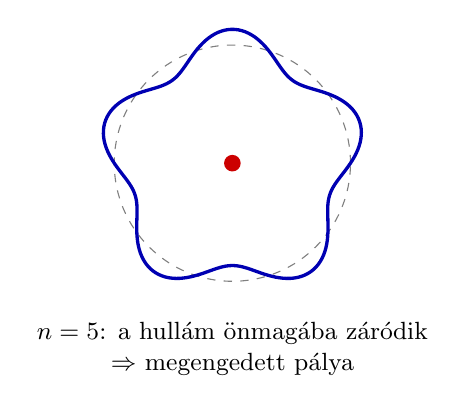
\begin{tikzpicture}[font=\small]
  \draw[gray,dashed] (0,0) circle (1.5);
  \fill[red!80!black] (0,0) circle (3pt);
  \draw[very thick,blue!70!black,domain=0:360,samples=240]
    plot ({(1.5+0.2*sin(5*\x))*cos(\x)},{(1.5+0.2*sin(5*\x))*sin(\x)});
  \node[below,align=center] at (0,-1.9) {$n = 5$: a hullám önmagába záródik\\$\Rightarrow$ megengedett pálya};
\end{tikzpicture}

\vspace{10pt}
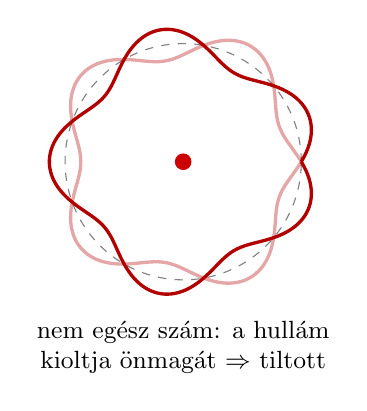
\begin{tikzpicture}[font=\small]
  \draw[gray,dashed] (0,0) circle (1.5);
  \fill[red!80!black] (0,0) circle (3pt);
  \draw[very thick,red!70!black,domain=0:360,samples=240]
    plot ({(1.5+0.2*sin(4.5*\x))*cos(\x)},{(1.5+0.2*sin(4.5*\x))*sin(\x)});
  \draw[very thick,red!70!black,domain=360:720,samples=240,opacity=0.35]
    plot ({(1.5+0.2*sin(4.5*\x))*cos(\x)},{(1.5+0.2*sin(4.5*\x))*sin(\x)});
  \node[below,align=center] at (0,-1.9) {nem egész szám: a hullám\\kioltja önmagát $\Rightarrow$ tiltott};
\end{tikzpicture}
\end{minipage}

%====================================================================
\dia{12. A kvantummechanikai atommodell (1925--1926)}

\begin{minipage}[t]{0.60\linewidth}\vspace{0pt}
\begin{itemize}
  \item \textbf{Schrödinger és Heisenberg:} az elektronnak \textbf{nincs pályája}. Az
    állapotát egy hullámfüggvény írja le, amely megadja, mekkora
    \textbf{valószínűséggel} találjuk az elektront egy adott helyen. Ennek képe az
    \textbf{elektronfelhő} (pálya helyett: \emph{atompálya, orbitál}).
  \item \textbf{Heisenberg-féle határozatlansági reláció:} az elektron helye és lendülete
    nem lehet egyszerre tetszőlegesen pontos:
    $\;\Delta x\cdot \Delta p \ge \dfrac{h}{4\pi}$. Ezért nincs értelme pontos pályáról
    beszélni.
  \item Az \textbf{energiaszintek megmaradnak}: a hidrogénre ugyanazt az
    $E_n = -13{,}6~\text{eV}/n^2$ képletet adja, de minden atomra működik.
  \item Az elektron állapotát \textbf{négy kvantumszám} adja meg: $n$ (fő-, a héj és az
    energia), $l$ (mellék-, a felhő alakja: s, p, d, f), $m$ (mágneses, a felhő iránya),
    $s$ (spin, $\pm\tfrac12$).
  \item \textbf{Pauli-elv:} egy atomban nem lehet két elektron, amelynek mind a négy
    kvantumszáma azonos. Ezért az $n$-edik héjon legfeljebb $2n^2$ elektron fér el
    ($2, 8, 18, \dots$). Ebből épül fel a \textbf{periódusos rendszer}: a kémiai
    tulajdonságokat a külső héj elektronjai szabják meg.
\end{itemize}
\end{minipage}\hfill
\begin{minipage}[t]{0.37\linewidth}\vspace{0pt}\centering
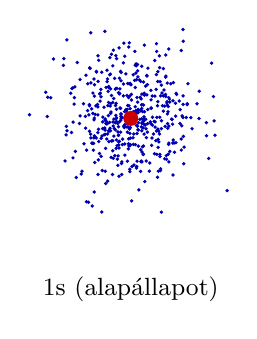
\begin{tikzpicture}[font=\small,scale=1.35]
  \felho{6000}{21}{exp(-(\x*\x+\y*\y)/0.18)}
  \fill[red!80!black] (0,0) circle (2pt);
  \node[below] at (0,-1.4) {1s (alapállapot)};
\end{tikzpicture}

\vspace{6pt}
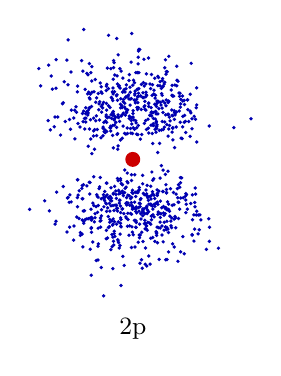
\begin{tikzpicture}[font=\small,scale=1.35]
  \felho{7000}{22}{(\y*\y/0.2)*exp(1-(\x*\x+\y*\y)/0.2)}
  \fill[red!80!black] (0,0) circle (2pt);
  \node[below] at (0,-1.4) {2p};
\end{tikzpicture}\\
{\scriptsize sűrűbb pontok: ott nagyobb valószínűséggel találjuk az elektront}
\end{minipage}

%====================================================================
\dia{13. Összefoglalás: modellek és kísérletek}

\begin{center}
\renewcommand{\arraystretch}{1.5}
\begin{tabular}{|>{\raggedright\arraybackslash}p{3.0cm}|>{\raggedright\arraybackslash}p{4.6cm}|>{\raggedright\arraybackslash}p{5.6cm}|>{\raggedright\arraybackslash}p{5.6cm}|}
\hline
\textbf{Modell} & \textbf{Kísérleti háttér} & \textbf{Mit magyaráz meg?} & \textbf{Mit nem?} \\ \hline
\textbf{Thomson} (1904) & katódsugárzás: az elektron felfedezése (1897); Millikan: elemi töltés
  & az atom semleges, és elektronok léphetnek ki belőle & az $\alpha$-részecskék nagy szögű szórását \\ \hline
\textbf{Rutherford} (1911) & $\alpha$-szórás aranyfólián (Geiger--Marsden)
  & az atommag létezését, a nagy szögű szórást & az atom stabilitását, a vonalas színképet \\ \hline
\textbf{Bohr} (1913) & vonalas színképek; Franck--Hertz-kísérlet (1914)
  & a hidrogén színképét, az ionizációs energiát, a diszkrét energiaszinteket
  & a többelektronos atomokat; miért éppen ezek a pályák \\ \hline
\textbf{kvantum\-mechanikai} (1926) & de Broglie, elektronelhajlás
  & minden atomot, a periódusos rendszert, a kémiai kötést & -- (ma is ezt használjuk) \\ \hline
\end{tabular}
\end{center}

\begin{minipage}[t]{0.55\linewidth}\vspace{0pt}
\begin{fontos}[title=Képletek,fonttitle=\bfseries]
$\dfrac{e}{m} = \dfrac{2U}{B^2r^2}$ \;(fonalsugárcső) \qquad
$q = \dfrac{mgd}{U} = n\cdot e$ \;(Millikan)\\[4pt]
$hf = E_\text{felső} - E_\text{alsó}$ \qquad $E_n = -\dfrac{13{,}6~\text{eV}}{n^2}$
\qquad $mvr = n\dfrac{h}{2\pi}$ \qquad $2\pi r = n\lambda$
\end{fontos}
\end{minipage}\hfill
\begin{minipage}[t]{0.42\linewidth}\vspace{0pt}
\begin{fontos}[colback=yellow!8,colframe=orange!70!black,title=Házi feladat,fonttitle=\bfseries]
A \emph{gyakorló feladatsor} feladatai, és szóbeli tétel: \emph{Az atommodellek
fejlődése} (3--4 perc).
\end{fontos}
\end{minipage}

\end{document}
